\section{Introdução ao Arduino}

\begin{frame}{O que é Arduino?}
  \begin{columns}
    \column{0.5\textwidth}
    \begin{itemize}
      \item Plataforma de prototipagem eletrônica
      \item Fácil de usar (hardware + software)
      \item Muito usada em:
            \begin{itemize}
              \item Robótica
              \item Automação
              \item IoT
            \end{itemize}
    \end{itemize}
    \column{0.5\textwidth}
    \begin{figure}
      \centering
      
\includegraphics[width=0.9\linewidth]{arduino/uno.jpg}
      \caption{Arduino Uno}
    \end{figure}
  \end{columns}
\end{frame}

\note{
  O Arduino é uma plataforma de prototipagem, ideal para testes e aprendizado.

  Em produtos finais, geralmente utiliza-se um circuito dedicado (com microcontrolador próprio), pois o Arduino pode não ser a solução mais otimizada em custo, tamanho e robustez.
}

\begin{frame}{Componentes do Arduino Uno}
  \begin{columns}
    \column{0.5\textwidth}
    \begin{itemize}
      \item Microcontrolador (ATmega328)
      \item Pinos digitais
      \item Pinos analógicos
      \item Porta USB
      \item Botão reset
      \item E muitos outros elementos
    \end{itemize}
    \column{0.5\textwidth}
    \begin{figure}
      \centering
      
\includegraphics[width=\linewidth]{arduino/parts.jpg}
      \caption{Componentes da placa Arduino Uno}
    \end{figure}
  \end{columns}
\end{frame}

\begin{frame}{PWM (Modulação por Largura de Pulso)}
  \begin{columns}
    \column{0.5\textwidth}
    \begin{figure}
      \centering
      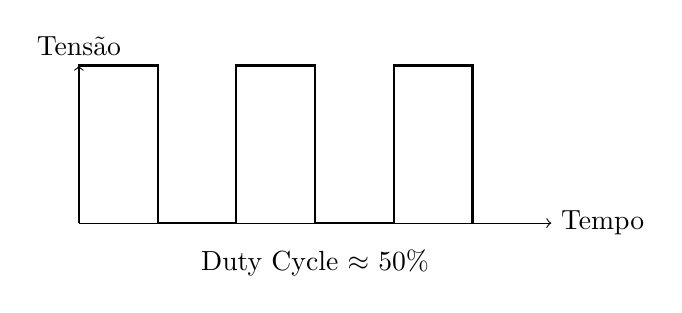
\begin{tikzpicture}
        \draw[->] (0,0) -- (6,0) node[right] {Tempo};
        \draw[->] (0,0) -- (0,2) node[above] {Tensão};
        % Sinal PWM
        \draw[thick] (0,0) -- (0,2) -- (1,2) -- (1,0) -- (2,0) -- (2,2) -- (3,2) -- (3,0)
        -- (4,0) -- (4,2) -- (5,2) -- (5,0);
        \node at (3,-0.5) {Duty Cycle $\approx$ 50\%};
      \end{tikzpicture}
      \caption{Exemplo de sinal PWM}
    \end{figure}
    \column{0.5\textwidth}
    \begin{itemize}
      \item Sinal digital que simula analógico
      \item Controla potência média
      \item Baseado em \textit{duty cycle}
    \end{itemize}
  \end{columns}
\end{frame}

\begin{frame}{Cuidados com o Arduino}
  \begin{block}{Limites Elétricos}
    \begin{itemize}
      \item Corrente por pino: \textbf{20 mA} (máx. 40 mA)
      \item Corrente total: \textbf{200 mA}
      \item Tensão máxima: \textbf{5V}
    \end{itemize}
  \end{block}
  \begin{columns}[T]
    \column{0.5\textwidth}
    \textbf{Evite:}
    \begin{itemize}
      \item Motores direto nos pinos
      \item Curto-circuito (VCC + GND)
    \end{itemize}
    \column{0.5\textwidth}
    \textbf{Use:}
    \begin{itemize}
      \item Resistores, LEDs
      \item Sensores, módulos..
    \end{itemize}
  \end{columns}
  \begin{alertblock}{Atenção}
    Ultrapassar esses limites pode queimar a placa!
  \end{alertblock}
\end{frame}

\begin{frame}{Tipos de Arduino}
  \begin{columns}[c]
    \column{0.33\textwidth}
    \begin{figure}
      \centering
      
\includegraphics[width=0.5\linewidth]{arduino/uno.jpg}
      \caption{Arduino Uno}
    \end{figure}
    \column{0.33\textwidth}
    \begin{figure}
      \centering
      
\includegraphics[width=0.5\linewidth]{arduino/nano.jpg}
      \caption{Arduino Nano}
    \end{figure}
    \column{0.33\textwidth}
    \begin{figure}
      \centering
      
\includegraphics[width=0.5\linewidth]{arduino/mega.jpg}
      \caption{Arduino Mega}
    \end{figure}
  \end{columns}
  \vspace{0.3cm}
  \begin{columns}[c]
    \column{0.2\textwidth}
    \column{0.3\textwidth}
    \begin{figure}
      \centering
      
\includegraphics[width=0.5\linewidth]{arduino/leonardo.jpg}
      \caption{Arduino Leonardo}
    \end{figure}
    \column{0.3\textwidth}
    \begin{figure}
      \centering
      
\includegraphics[width=0.5\linewidth]{arduino/lilypad.png}
      \caption{Arduino Lilypad}
    \end{figure}
    \column{0.2\textwidth}
  \end{columns}
\end{frame}

\begin{frame}{Arduino IDE}
  \begin{figure}
    \centering
    
\includegraphics[width=0.8\linewidth]{ide.png}
    \caption{Ambiente para escrever, compilar e enviar programas para o Arduino.}
  \end{figure}
\end{frame}
